% !TEX program = pdflatex
\documentclass[tikz,border=3mm]{standalone}
\usepackage{amsmath,amssymb}
\usepackage{mathrsfs}
\usepackage{tikz}
\usetikzlibrary{arrows.meta,calc,positioning,fit,backgrounds,decorations.pathreplacing,shapes.geometric}

% --- your color definitions and macros here (paste exactly from your code) ---

\begin{document}
% --- paste your full \begin{tikzpicture} ... \end{tikzpicture} here (unchanged) ---
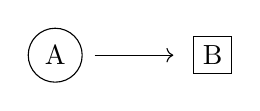
\begin{tikzpicture}
  % Example content
  \node[draw, circle] at (0,0) {A};
  \node[draw, rectangle] at (2,0) {B};
  \draw[->] (0.5,0) -- (1.5,0);
\end{tikzpicture}
\end{document}
